\section{Problem statement}
\label{sec:problem_statement}

The task of detecting and tracking moving targets is non-trivial. There are many sources of tracking errors, including raw sensor data noise, illumination levels, changing backgrounds, and occlusion. Real-world environments are unpredictive and complex, thus making the task much harder. The system attempts to solve the problme of occlusion with multiple Kinects.

Occlusion occurs when the tracked target is masked by other objects in the scene. The masked target would not exist in the field of view of one or more cameras. If a person were occluded, his precise joint positions and movements would be unknown. Resolving the problem of occlusion would provide any tracking system with more spatial and physiological information about the tracked people.

There are two types of occlusions. Static occlusion refers to occlusion caused by stationary objects, and dynamic occlusion refers to occlusion arised from interactions of many targets in the environment. The aim is to resolve both types of occlusion.

A simple instance of the problem is illustrated in Figure \ref{fig:occlusion_problem}. In the figure, both skeletons are invisible to the front Kinect but visible to the side Kinect. They are occluded by the red obstacle. When they step out of the obstacle into the views of both Kinects, the system should merge the skeletons of the same person from different perspectives. The main objective of the project is to avoid occlusion by extending the field of view of the system. The proposed algorithm would combine depth sensor information from multiple Kinects to achieve this goal.

\begin{figure}[h!]
  \centering
  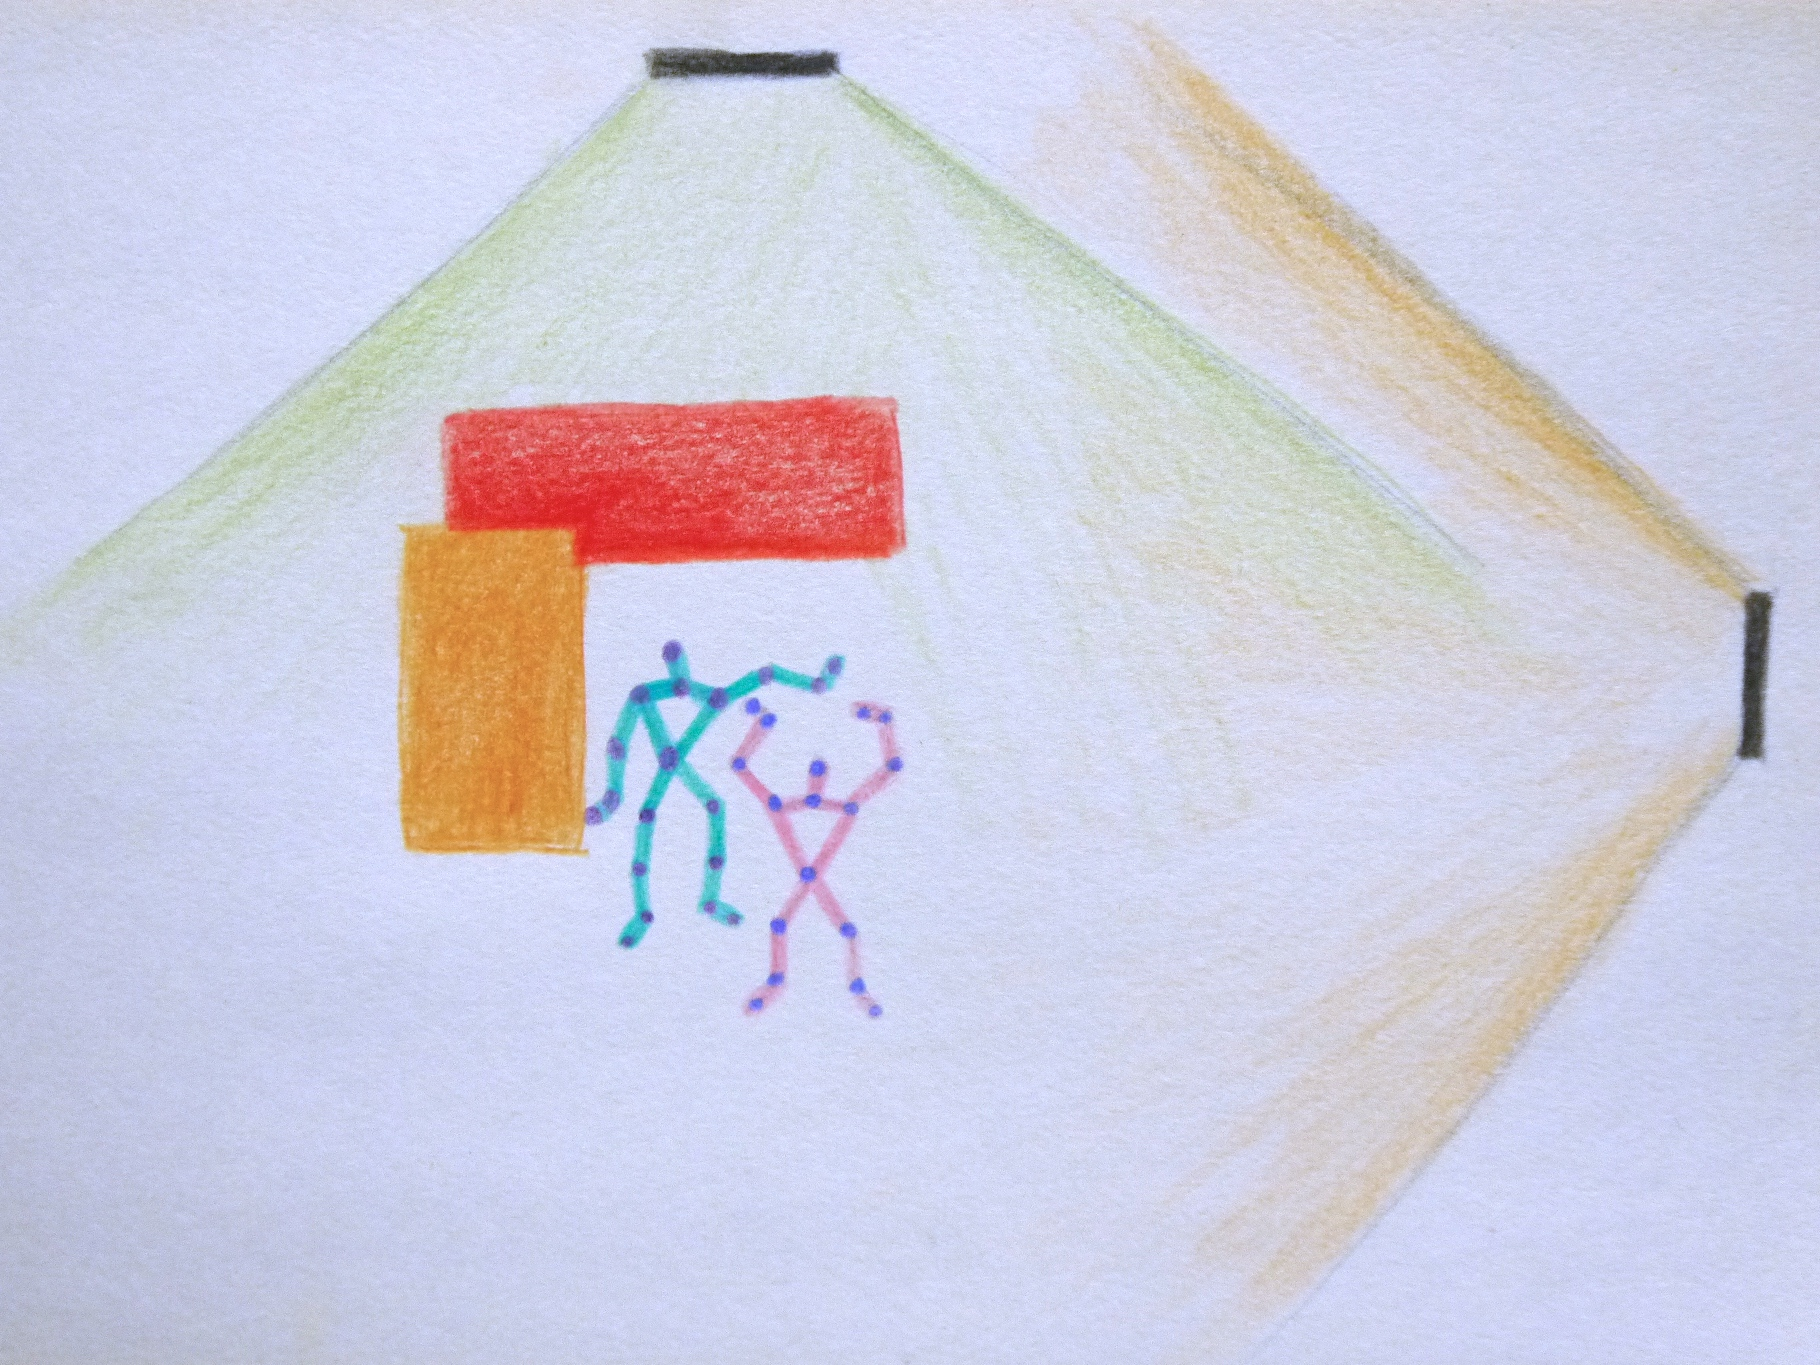
\includegraphics[width=0.9\columnwidth]{occlusion_problem}
  \caption{The occlusion problem}
  \label{fig:occlusion_problem}
\end{figure}

\subsection{Aims and Objectives}

\textbf{TODO}
